
\section{Event reconstruction and selection} 

The \minerva\ detector records the charge and time of energy
depositions (hits) in each scintillator strip.  Hits are first grouped
in time and then clusters of energy are formed by spatially grouping
adjacent hits in each scintillator plane.  Clusters with energy
more than $\unit[1]{MeV}$ are then matched among the three views to create a
track. The per-plane position resolution is 2.7~mm and the
angular resolution of the muon track is better than
10~mrad~\cite{minerva_nim} in each view. The $\mu^+$ is identified by matching a
track that exits
the back of \minerva with a positively-charged track entering the
front of \minos. The reconstruction of the muon in the MINOS spectrometer gives
a typical momentum resolution of $11\%$. 
Event pile-up causes a decrease in the muon track reconstruction efficiency. 
This effect is studied in both \minerva and \minos by projecting tracks found in
one of the detectors to the other and measuring the mis-reconstruction rate. 
This results in a $-4.4\%$ ($-1.1\%$) correction to the simulated efficiency for
muons below (above) 3 GeV/c.

The event vertex, defined as the most upstream cluster on the muon track, is restricted to be
within the central 108 planes of the scintillator tracking region and
no closer than \unit[22]{cm} to any edge of the planes. These
requirements define a fiducial volume with a mass of \unit[5.47]{metric tons}.
%There are eight tracking planes between the fiducial volume and the most downstream
%of the passive nuclear targets, and eight tracking planes between the fiducial volume and
%the start of the electromagnetic calorimeter. 
Due to the requirement that the $\mu^+$ is tracked in MINOS for charge and momentum
measurement, the detection efficiency has a strong dependence on muon angle $\theta_\mu$ and
momentum $|\vec{p}_\mu|$, which drops to zero for  events with  $\theta_\mu$ greater than
$\unit[20]{degrees}$ or $|\vec{p}_\mu|$ less than $\unit[1.0]{GeV/c}$.
The corrections for the angle and momentum efficiency are estimated
from the event simulation. Only events with a single track at the vertex,
 the $\mu^+$ matched to MINOS, are used in order to reject events including
 charged pion production. 
Accepted events are passed to the $\pi^0$ reconstruction.  

The neutral pion has a lifetime of $\unit[8.52\times10^{-17}]{s}$ and decays
into two photons with a branching ratio of 98.8\%~\cite{pdg}, so the two photons appear
to come from the event vertex. 
Plastic scintillator has a radiation length $X_0\sim\unit[40]{cm}$, which
allows the two photons to convert by $e^+e^-$ pair production or Compton
scattering 
far away from the vertex, thus producing isolated energy deposits. 
The photons can also have significant energy leakage or escape the detector
without conversion. 
Furthermore, energy deposits produced by neutrons from the same neutrino
interaction can be mistaken for low-energy photon conversions, further
complicating the pattern of energy deposits. 
The $\pi^0$ reconstruction must correctly group these energy deposits into
the two photons. 


The reconstruction can be separated into two steps: pattern recognition and
kinematic reconstruction. The pattern recognition builds upon the knowledge of the vertex
location of the event. In the X view, clusters that are close in polar angle with respect to
the vertex but can be
separated in radial distance from the vertex are grouped into photon candidates. 
Then, for each candidate, clusters in the U and V views consistent with the stereo condition are added. 
Photon candidates must have clusters from at least two views
for three-dimensional direction reconstruction.


In the second step, photon position, direction, and energy are determined from
the clusters that have been assigned to the photons. 
The photon direction is reconstructed from the cluster energy-weighted slopes in each view.
The photon vertex is defined by the closest cluster to the event
vertex on the photon direction axis. 
The photon energies are reconstructed by calorimetry using calibration constants 
determined from the simulation. 
The overall calibration constant that sets the absolute energy scale is
determined by matching the peak in the $\gamma\gamma$ invariant mass
distribution to the $\pi^0$ nominal mass of
$\unit[134.97]{MeV/c^2}$~\cite{pdg}. 
This procedure is done separately for data and simulation which enables
correction for a difference in energy scales of 5\% between the data and simulation. 
Finally, the $\pi^0$ momentum is calculated from momentum conservation, $\vec p_{\pi^0}
= \vec{k}_1 + \vec{k}_2$, where $\vec{k}_i$ % = \vec{k}_i(E_i, \theta_i, \phi_i)$
are reconstructed photon momenta. 
The $\pi^0$ is reconstructed with a 25\% energy resolution and
$\unit[3.5]{degrees}$ angular resolution in each view. The incoming neutrino energy is
reconstructed from the $\mu^+$ and $\pi^0$ 4-momenta using
\begin{eqnarray}
 E_\nu^{rec} &=& E_\mu + E_{\pi^0} + T_n \\ \nonumber
 T_n &=& \frac{1}{2}\frac{[(E_\mu-p_\mu^\parallel)+(E_{\pi^0}-p_{\pi^0}^\parallel)]^2 + (\vec{p}_\mu^\perp + \vec{p}^\perp_{\pi^0})^2}
 {m_N-(E_\mu-p_\mu^\parallel)-(E_{\pi^0}-p_{\pi^0}^\parallel)},
\end{eqnarray}
where $\vec{p}^\perp, p^\parallel$ are the transverse and longitudinal components of momentum, respectively. 
It is assumed that the initial nucleon is at rest and that the $\pi^0$ is produced
together with a nucleon. The neutrino energy is reconstructed with 10\% resolution.
The $\gamma\gamma$ invariant mass $m_{\gamma\gamma}$ is reconstructed from the photon energies $E_{1,2}$ and
the separation angle $\theta_{\gamma\gamma}$ between the two photons using
\begin{equation}
m_{\gamma\gamma}^2=2E_1E_2(1-\cos\theta_{\gamma\gamma}). 
\end{equation}

The two reconstructed photons are required to convert at least $\unit[15]{cm}$ ($0.36X_0$) away
from the vertex to further reject charged-pion backgrounds. 
In addition, it is required that $E_\nu^{rec}$ is between 1.5 and 20 GeV.
The lower energy cut is needed due to MINOS acceptance while the upper cut is to reduce flux uncertainties.
Finally, it is required that $m_{\gamma\gamma}$ is between
$\unit[75]{MeV/c^2}$ and $\unit[195]{MeV/c^2}$. 
The selected sample has 1304 events. 
The total selection efficiency is 6\% and
purity 55\%, according to the simulation. 
The background is dominated (70\% of the total background) by events with at
least one $\pi^0$ in the detector. 
Half of this is due to multi-pion production, $\pi^0+\pi^{\pm}$,
where the $\pi^{\pm}$ is not tracked, while 
the other half has a secondary $\pi^0$ produced by $\pi^-\rightarrow\pi^0$ CEX 
or nucleon scattering in the detector but outside the primary
interaction nucleus. 
The non-$\pi^0$ background is mostly due to energy deposits by $\pi^-$ and neutrons
which are mistakenly
identified as photons, and accounts for the remaining 30\% of the total
background.

Figure \ref{fig:invariant-mass} shows the $m_{\gamma\gamma}$
distributions for both data and simulation of the selected sample before the
invariant mass cut. 
There is a clear peak centered around the $\pi^0$ nominal mass in both data and
simulation. 
The distribution from simulation is broken down into signal and background
components. The signal is defined as antineutrino 
charged-current events with single $\pi^0$ and no $\pi^\pm$ escaping 
the nucleus. The background is anything else that is not signal. By this definition, 
it is possible for signal events to have the $\pi^0$s mis-reconstructed from non-$\pi^0$ energy 
deposits. The signal events at high $m_{\gamma\gamma}$, outside the signal mass width, have one or 
both candidate photons reconstructed from neutron energy deposits. 
The same mis-reconstruction happens to signal events in the selected sample but at a smaller rate (14\%). 
The $\pi^0$ momentum and angular shapes of these events are found to be similar to the rest of the signal events.
The enhancement in the background distribution around the $\pi^0$
mass is due to background events with at least one $\pi^0$ in the
detector. 

After event selection, the selected
sample still has substantial background to be subtracted statistically
from the total distribution for each observable. 
The background distribution for each observable is estimated from the simulation
with the total background rate constrained by data. 
This significantly reduces the uncertainties in the estimated background. 
The background rate is determined from a binned extended maximum likelihood
fit of an invariant mass model to the data~\cite{Barlow:1993dm}. 
The invariant mass model $M(m_{\gamma\gamma})$ is a two-component model
constructed from the $m_{\gamma\gamma}$ distributions of signal and background
events,
\begin{equation}
M(m_{\gamma\gamma})=N_{sig}M_{sig}(m_{\gamma\gamma}) +
N_{bkg}M_{bkg}(m_{\gamma\gamma}),
\end{equation}
where $M_{sig}(m_{\gamma\gamma}), M_{bkg}(m_{\gamma\gamma})$ are the shapes of
the signal and background $m_{\gamma\gamma}$ distributions from the simulation, respectively. 
The expected numbers of signal and background events $N_{sig},N_{bkg}$ in the
range 0-500 MeV/$c^2$ are the parameters determined from the fit. 
After the fit, a background rate of 541$\pm$37 events is obtained by integrating
the curve $N_{bkg}M_{bkg}(m_{\gamma\gamma})$ over the mass peak region from
$\unit[75]{MeV/c^2}$ to $\unit[195]{MeV/c^2}$, the same range as required by the event selection.
The fit reduces the background normalization by a factor of 0.8 compared to the simulation prediction.

\begin{figure}[!htpb]
\centering
\ifnum\PLsupp=0
  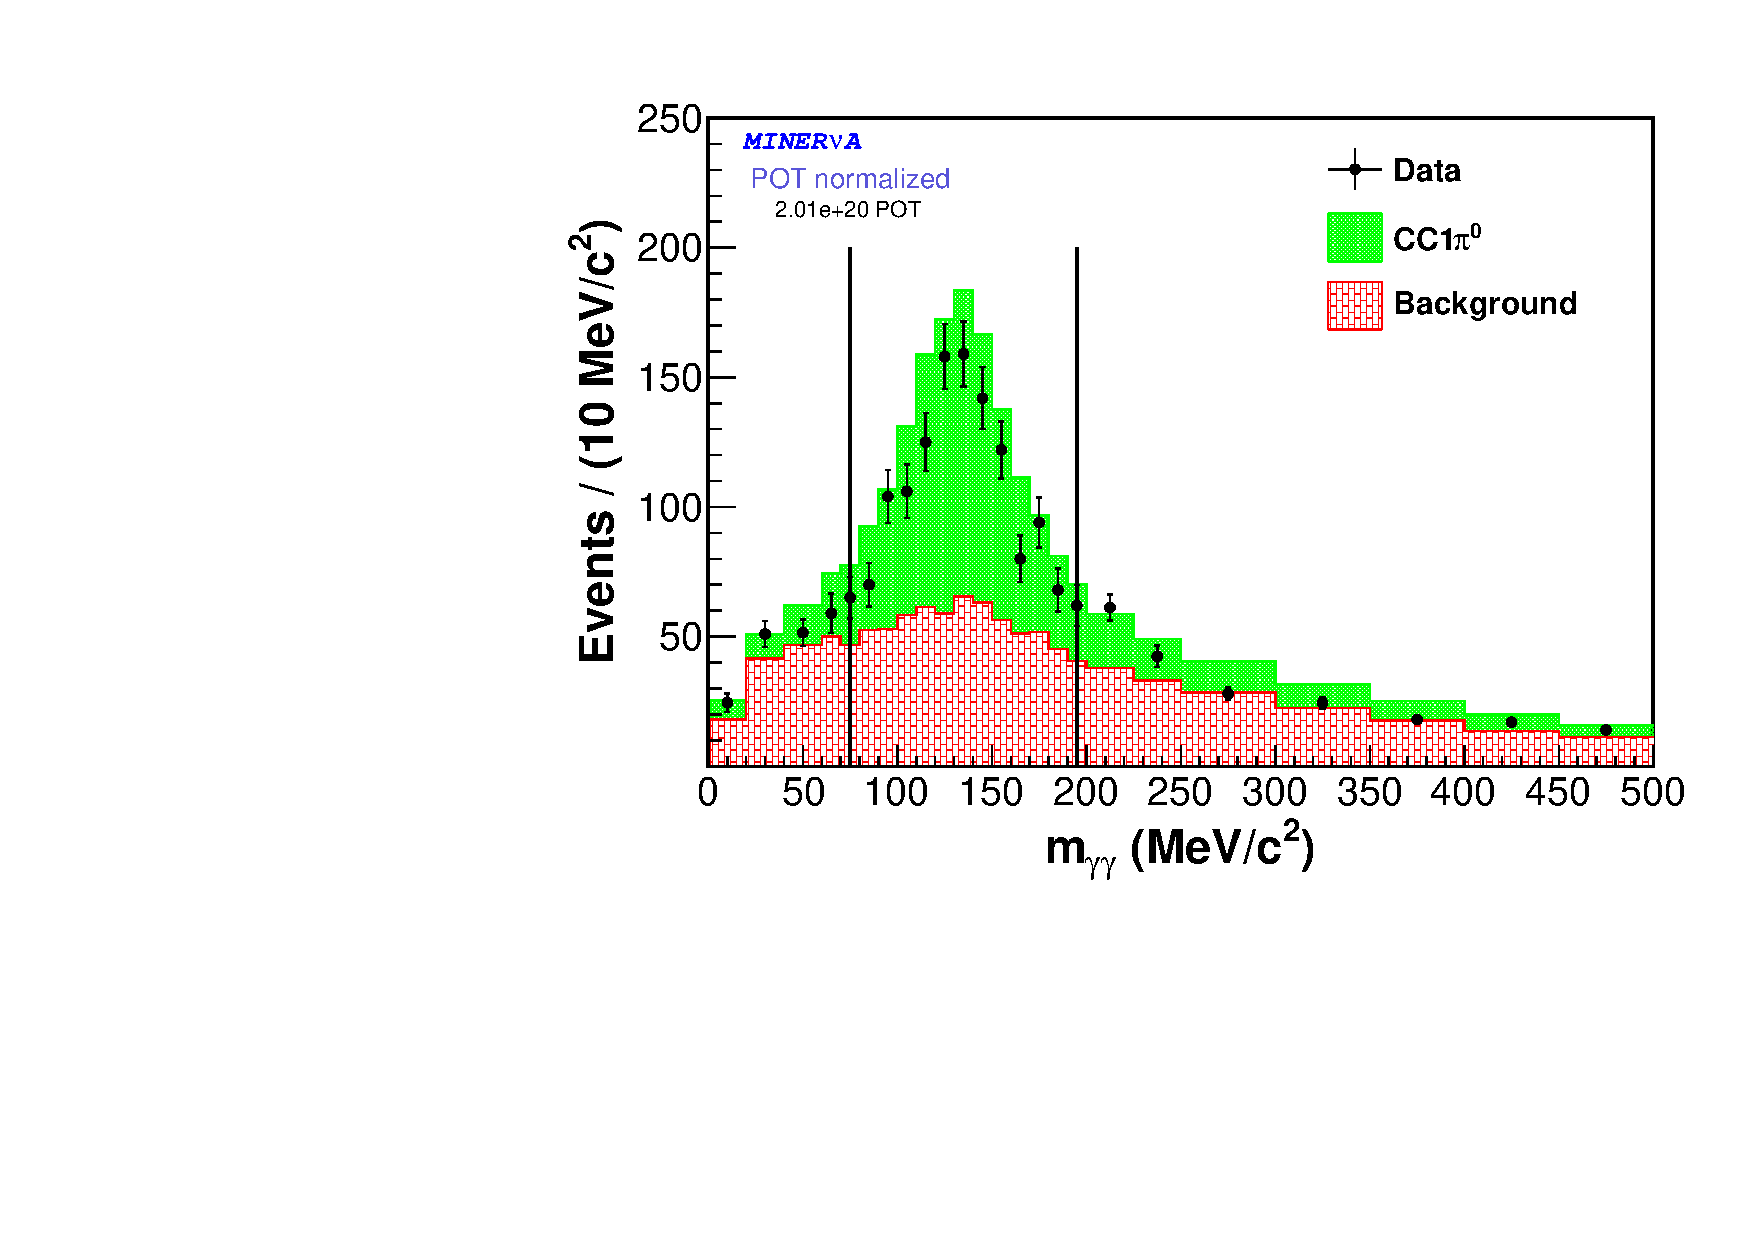
\includegraphics[width=1.0\columnwidth]{mgg-data-mc-breakdown-pot.pdf}
\else
  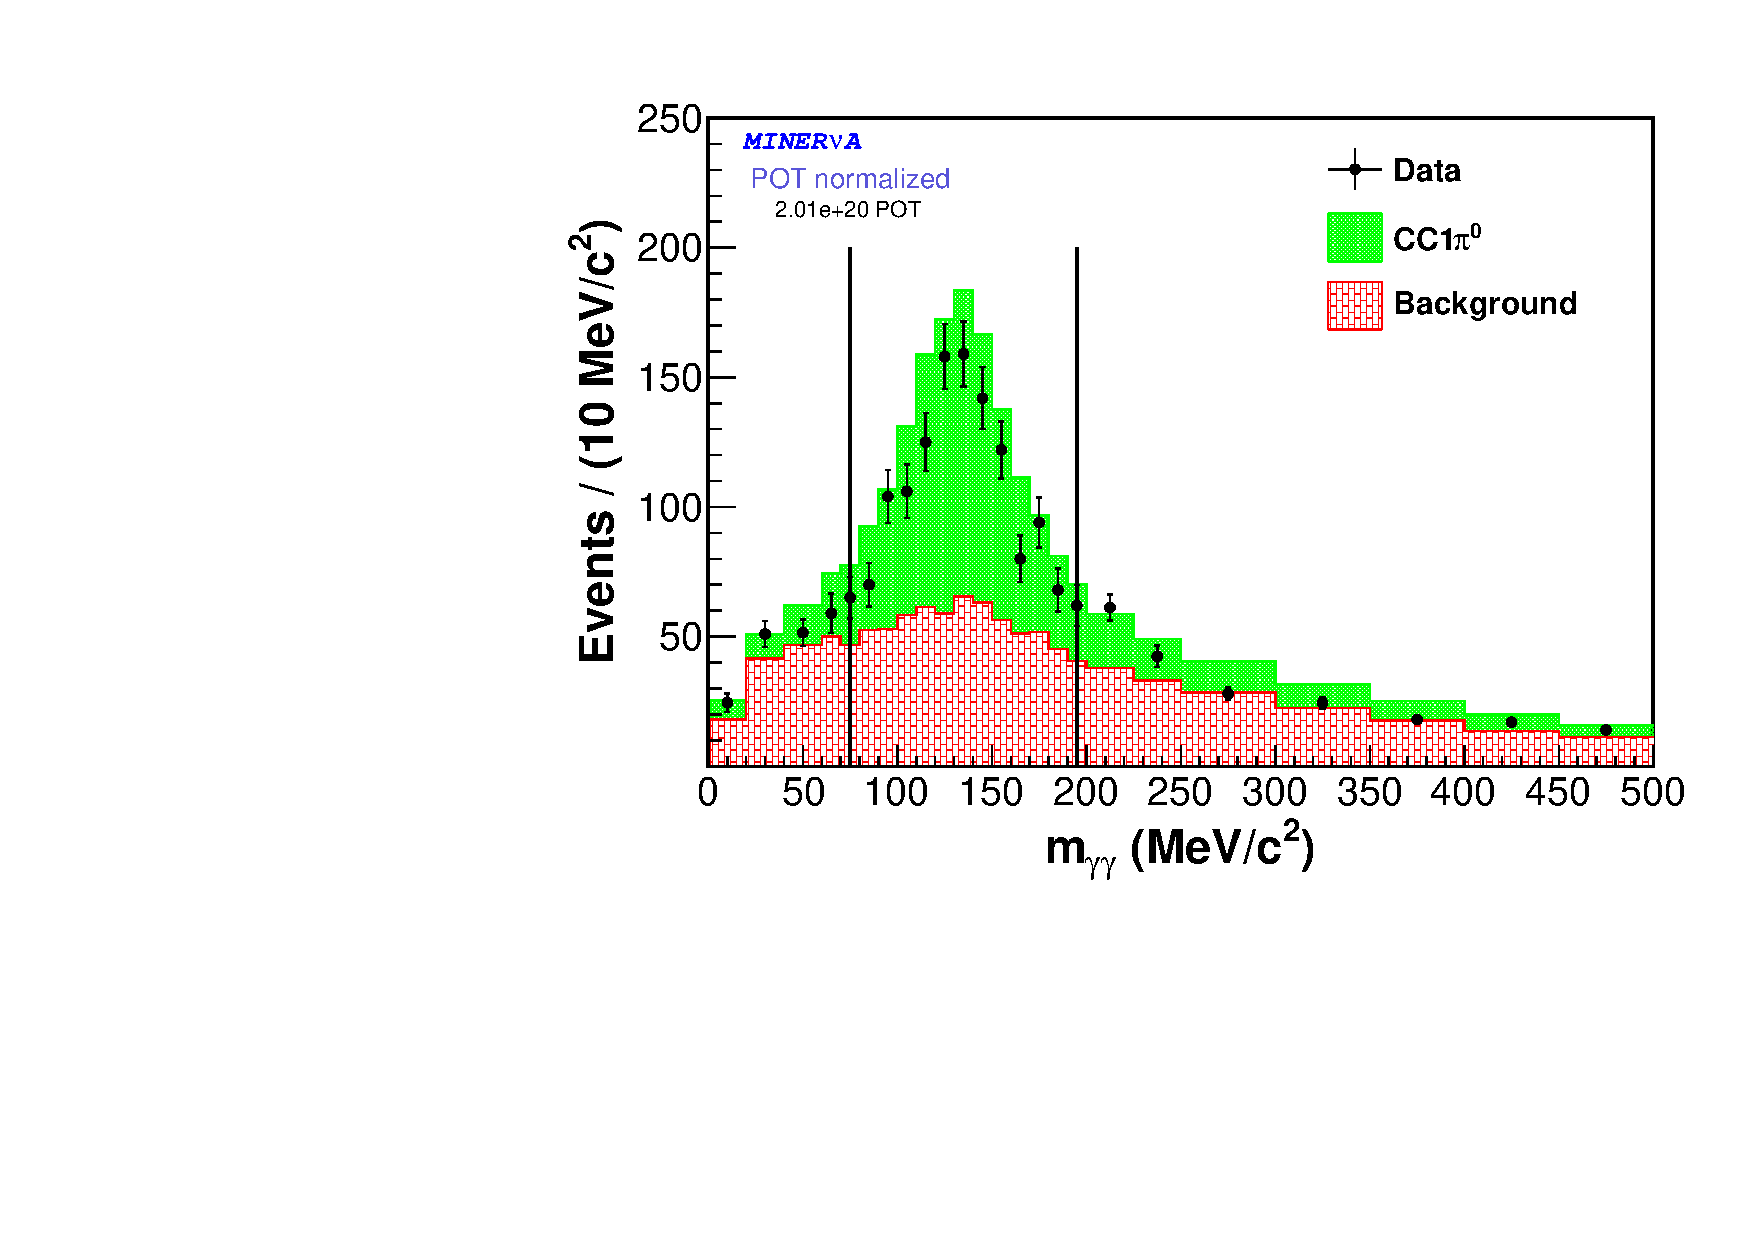
\includegraphics[width=1.0\columnwidth]{mgg-data-mc-breakdown-pot.pdf}
\fi

\vspace{-7pt}

\caption{Distribution of the invariant mass of the $\gamma\gamma$ pair.
Data are shown as solid circles with statistical error bars. 
The shaded histograms show the Monte Carlo predictions for CC1$\pi^0$ signal (top) and for background (bottom). 
The signal is defined as antineutrino charged-current events with single $\pi^0$ and no $\pi^\pm$ escaping 
the nucleus. The background is anything else that is not signal. 
The vertical lines indicate the invariant mass cut, $\unit[75]{MeV/c^2} < m_{\gamma\gamma} < \unit[195]{MeV/c^2}$.}
\label{fig:invariant-mass}
\end{figure}

The estimated background is subtracted from the total distribution. This
background-subtracted data distribution is unfolded to account for detector
resolution effects 
using a Bayesian unfolding method~\cite{agostini:1995} with two iterations. 
The migration matrix used in the unfolding is obtained from the simulation. 
The reconstruction efficiency and acceptance corrections are made by dividing by
an efficiency curve derived from the simulation. 
Dividing this corrected distribution by the integrated flux
($2.5\times10^{-8}\bar{\nu}_\mu/\text{cm}^2/\text{POT}$) of antineutrinos with
energies in the range 1.5-20 GeV, 
and the number of nucleons in the fiducial volume ($3.30\times10^{30}$) gives
the differential cross section. 

